\section{Plasma Oscillation}
	\label{sec:langmuir_verification}
	As a test of the validity of our PiC program, we can use the Langmuir
	oscillation, described in \cref{sec:langmuir}.
	This test is inspired by a case set up in \citet{birdsall_plasma_2004},
	and modified to fit with our normalization and discretizations.
	To verify that the oscillation is properly simulated we will look at oscillations in the energy.


    \subsection{Input parameters}
        \subsubsection{Timestep}
        First we need to ensure that the simulation is does not violate the time-
        stability criterion, \cref{sec:time_stability}, \(\Delta t \leq 2\omega_{pe}\).
        For computational reasons each particle in the program represents many real particles
        and we can adjust the number, of real particles represented, to ensure
        that the electron plasma frequency is \(1\).

        \begin{equation}
            \omega_{pe}^2 = \frac{nq^2_e}{m\epsilon_0} = \left(\frac{N}{V}\right)\left(\frac{q_{e*}}{m_{e*} }\right)q_{e*}
        \end{equation}

        Here \((N/V)\) is just the number of electron super-particles divided by the volume,
        \(q_e\) and \(m_e\), represents super-particles and needs to be multiplied by the number
        of particles in a super-particle, \(\kappa\).

        \begin{equation}
            \omega_{pe}^2 = \left(\frac{N}{V}\right)\left(\frac{e}{m_e}\right)\kappa e
        \end{equation}

        Since we want the electron plasma frequency to be \(1\), \(\kappa\) is set to

        \begin{equation}
            \kappa = \frac{Vm_e}{Ne^2}
        \end{equation}

        Now the time is given in units of \(\omega_{pe}\) and we use \(\Delta t = 0.2 < 2\) easily.

        \subsubsection{Spatial-step}
        The spatial step need to satisfy the finite grid instability condition,
        \(\Delta x < \varsigma \lambda_{Se}\), \cref{sec:finite_grid_instability}.
        We use a similar procedure as in normalizing the time with regards to \(\omega_{pe}\)
        to normalize the length with regards to \(\lambda_{Se}\). The we end up with
        the temperature, or its other representation as thermal velocity, as the parameter we can adjust to make sure that it satisfies the
        condition.

        \begin{equation}
            \lambda_{Se}^2 = \frac{\epsilon_0 kT_e}{nq^2_e}
        \end{equation}

		% To make sure that

		\subsubsection{Simulation}
			We ran a simulation for \(10\tau_{pe}\), on a \(64,64,64\) size grid. The particles
			was first randomly distributed and given a maxwellian velocity distribution.
			Then they were slightly perturbed to create an imbalance.

			\begin{table}
					\center
			\begin{tabular}{c|c|c|c|c}
				Size 			&	Stepsize &	Timestep &\#Particles per cell	& \(v_{th}\) (electrons, ions)
				\\ \hline
				\((64,64,64)\)	& \(0.2\)	& \(0.1\)  	&	\(64\)	& 		\(0.002, 0.00046\)
			\end{tabular}
			\caption{Key settings for the langmuir wave oscillation. The complete settings are
			stored as an input file, langmuirWarm, in the PINC directory.}
			\end{table}

			The simulation were set to run for \(100\) timesteps, where each timestep represents \(0.1omega_{pe}^{-1}\).
			\begin{equation}
				\tau_p \equiv 2\pi/\omega_{pe}
			\end{equation}
			Using the plasma period this gives \(10/2\pi\approx 1.6\) periods.

		\begin{figure}
			\label{fig:oscillation}
			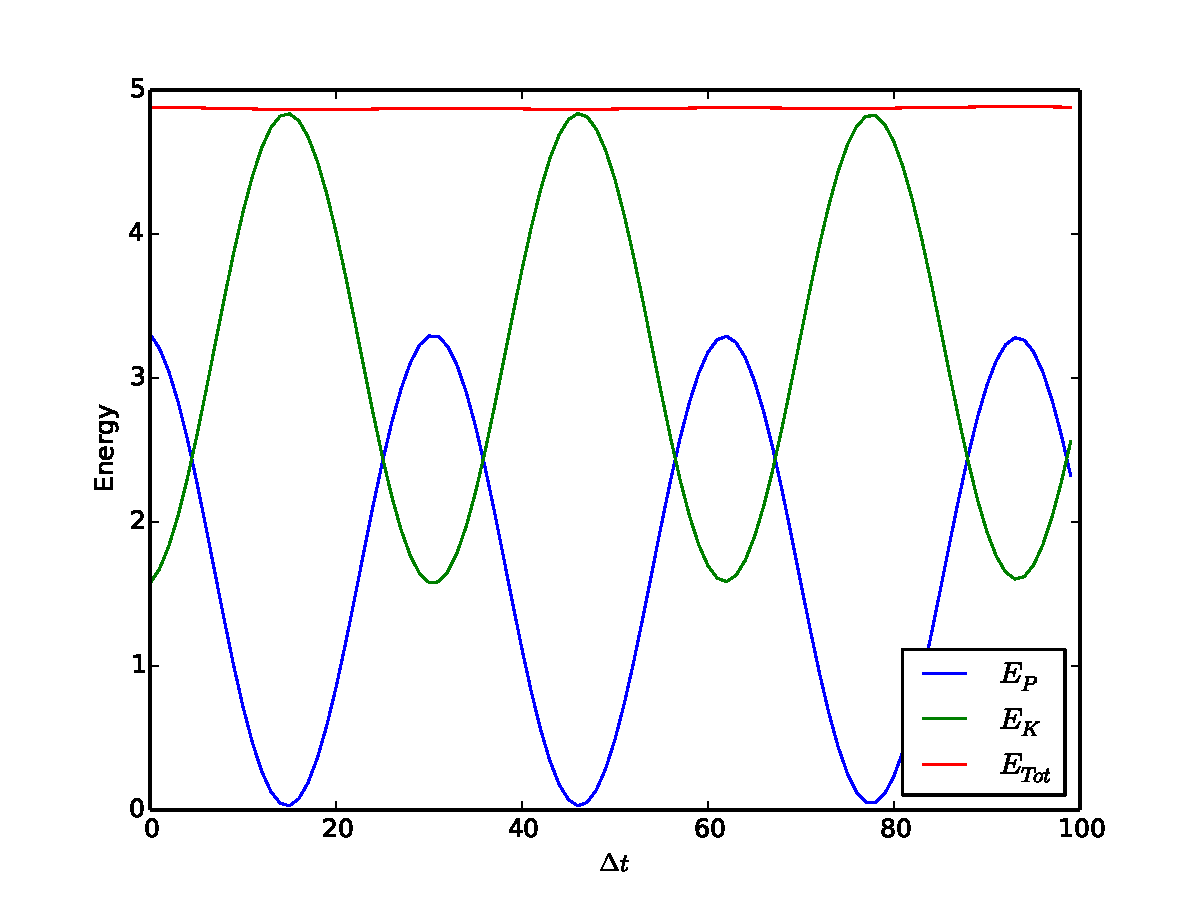
\includegraphics[width = \textwidth]{figures/verification/langmuirWave/energyPlot}
			\caption{This shows the time-evolution of the energy in an perturbed plasma. The energies are
			in normalized units and \(\Delta x = 0.1 \lambda_{De}\). The total energy has a maximum variation of \(0.22\%\). In the timespan
			of \(10\omega_{pe}\) the plasma oscillates over \(1.6\) times.}
		\end{figure}

		The \cref{fig:oscillation} shows the energy fluctuations for a plasma oscillation, the total energy
		is stable conserved, with a maximal variation of \(0.22\%\). The potential energy starts large
		and then it sinks as the potential energy is converted to kinetic energy. This is due to the particles
		attempting to neutralize the fields. The particles overshoots equilibrium position and the kinetic
		energy starts to convert back to potential energy.
